% !TeX program = xelatex
% !TeX program = xelatex
% ===========================================================================
%  tech_common.tex -- 两份技术文档共用的导言区
% ===========================================================================
\documentclass[11pt,a4paper]{ctexart}

\usepackage[top=2.4cm,bottom=2.4cm,left=2.4cm,right=2.4cm]{geometry}
\usepackage{amsmath,amssymb,amsthm}
\usepackage{graphicx}
\usepackage{booktabs}
\usepackage{longtable}
\usepackage{array}
\usepackage{enumitem}
\usepackage{xcolor}
\usepackage{listings}
\usepackage{tcolorbox}
\usepackage{caption}
\usepackage{fancyhdr}
\usepackage{titlesec}
\usepackage{hyperref}

\hypersetup{colorlinks=true,linkcolor=blue!55!black,citecolor=blue!55!black,
            urlcolor=blue!55!black,bookmarksnumbered=true}

% ---------------------------------------------------------------- 字体/版式
\setlength{\emergencystretch}{2.5em}
\setlength{\parskip}{0.35em}
\setlength{\parindent}{2em}
\linespread{1.12}

% ---------------------------------------------------------------- 代码样式
\definecolor{codebg}{RGB}{247,247,250}
\definecolor{codekw}{RGB}{0,90,160}
\definecolor{codecm}{RGB}{0,128,96}
\definecolor{codest}{RGB}{170,60,60}
\lstset{
  basicstyle=\ttfamily\footnotesize,
  backgroundcolor=\color{codebg},
  frame=single, framerule=0.4pt, rulecolor=\color{gray!45},
  breaklines=true, breakatwhitespace=false,
  numbers=left, numberstyle=\tiny\color{gray!80}, numbersep=6pt,
  keywordstyle=\color{codekw}\bfseries, commentstyle=\color{codecm}\itshape,
  stringstyle=\color{codest}, showstringspaces=false, columns=flexible,
  tabsize=2, extendedchars=true, captionpos=b,
  xleftmargin=1.6em, framexleftmargin=1.4em
}
\renewcommand{\lstlistingname}{代码}

% ---------------------------------------------------------------- 提示框
\newtcolorbox{keybox}[1][]{colback=blue!4,colframe=blue!45!black,
  boxrule=0.6pt,arc=2pt,left=5pt,right=5pt,top=4pt,bottom=4pt,
  fonttitle=\bfseries,#1}
\newtcolorbox{warnbox}[1][]{colback=orange!6,colframe=orange!55!black,
  boxrule=0.6pt,arc=2pt,left=5pt,right=5pt,top=4pt,bottom=4pt,
  fonttitle=\bfseries,#1}

% ---------------------------------------------------------------- 定理环境
\newtheorem{theorem}{定理}
\newtheorem{proposition}{命题}
\newtheorem{lemma}{引理}
\renewcommand{\proofname}{\heiti 证明}

% ---------------------------------------------------------------- 页眉页脚
\pagestyle{fancy}
\fancyhf{}
\fancyhead[L]{\small\color{gray!70}\leftmark}
\fancyhead[R]{\small\color{gray!70}\thepage}
\renewcommand{\headrulewidth}{0.3pt}
\renewcommand{\headrule}{\hbox to\headwidth{\color{gray!40}\leaders\hrule height \headrulewidth\hfill}}

\titleformat{\section}{\normalfont\heiti\Large}{\thesection}{0.6em}{}
\titleformat{\subsection}{\normalfont\heiti\large}{\thesubsection}{0.6em}{}
\titleformat{\subsubsection}{\normalfont\heiti\normalsize}{\thesubsubsection}{0.6em}{}

\captionsetup{font=small,labelfont=bf,labelsep=quad}


\title{\heiti 问题三技术报告\\[4pt]
       \large 全向干扰源的自动搜索、定位与清除\\[2pt]
       \normalsize —— 我是怎么做的：模型、算法、实现、实验与调试全过程}
\author{2026 高教社杯全国大学生数学建模竞赛 B 题}
\date{\today}

\begin{document}
\maketitle
\thispagestyle{fancy}

\begin{abstract}
\noindent
本文档记录问题三（目标区域内全部为全向干扰源，总数 10$\sim$16 个未知）的完整解决过程：
题面约束的逐条梳理、三个核心判断（真实时间不构成瓶颈、移动是主要成本、必须同时解决
"保证发现/可证终止/在线路径"）、信息模型与决策模型的建立、四阶段算法（普查—机会式交会—
射线归航—可证终止）的详细设计、与附件 1/2 协议一致的本地模拟器实现、60 组演练测试与
3 次正式测试的完整数据，以及开发过程中**真实出现并修复的 6 个故障**。

最终结果：60 组演练测试\textbf{完成率 100\%}、平均定位清除时间 \textbf{328.0 s}；
三次正式测试分别清除 15/15、12/12、10/10 个干扰源，平均定位清除时间
274.4 s、378.4 s、369.0 s，程序运行时间均小于 2 s（上限 20 min）。
\end{abstract}

\tableofcontents
\newpage

% ===========================================================================
\section{题面约束梳理}

\subsection{题目给出的条件}

\begin{longtable}{p{3.4cm}p{11.4cm}}
\toprule
项目 & 内容 \\ \midrule
\endhead
目标区域 & 半径 1800 m 的圆域，圆心为原点，$x$ 正东、$y$ 正北，单位 m \\
干扰源 & 全为\textbf{全向}源；总数 $10\sim16$ 但\textbf{具体个数未知}；位置在区域内均匀随机 \\
频道 & 每个源频道互不相同，取自 $\{1,\dots,20\}$，不随时间变化；不同源信号互不影响 \\
有效接收半径 & 每个源各不相同，取值在 $1000\sim1500$ m \\
示向度误差 & 与真实方位角之差 $\in[-1^{\circ},1^{\circ}]$；\textbf{同一地点固定}，重复检测不改变结果 \\
机器狗 & 从原点 $(0,0)$ 出发；测向机初始频道为 1；沿直线以 5 m/s 移动 \\
计时 & 移动 $=$ 距离$/5$ s；任意两频道切换 1 s；一次检测 5 s；清除命中 5 s、未命中 3 s \\
清除条件 & 距源 $\le20$ m 即可清除，与角度无关；同一源只能清除一次 \\
“near” & 距源 $\le5$ m 且在覆盖角内时无法给出示向度，可直接清除 \\
程序运行时间 & 上限 20 min（真实时间）；虚拟世界活动时长上限 100 h \\
\bottomrule
\end{longtable}

\subsection{需要交付的两个统计量}

\begin{equation}
\begin{aligned}
\text{被清除干扰源个数的比例}&=\frac{\text{被清除干扰源的个数}}{\text{干扰源总数}},\\[2pt]
\text{平均定位清除时间}&=\frac{\text{定位清除总时间}}{\text{被清除干扰源的个数}} .
\end{aligned}
\end{equation}

其中"定位清除总时间"含移动、频道切换、检测、光学精确定位与清除的全部耗时。
第一个指标要求\textbf{不漏源}，第二个指标要求\textbf{快}——两者共同决定了模型必须同时具备
"保证发现"与"可证终止"两个能力。

% ===========================================================================
\section{我的三个核心判断}

\subsection{判断一：真实时间从来不是瓶颈，优化目标是虚拟时间}

20 min 的程序运行时间限制作用在\textbf{真实时间}上。本地模拟中一次 HTTP 请求的往返时间约
1 ms，而它在虚拟世界里推进 5$\sim$100 s。60 组演练中单局程序运行时间均小于 0.6 s，
距离 1200 s 的上限有三个数量级的余量。

\begin{keybox}[title=结论]
既然真实时间不是约束，就应该把全部算力投入到\textbf{虚拟时间}的优化上：可以在每一步做
最近邻$+$2-opt 重规划、可以在线做认证检测，都不必担心算不过来。
\end{keybox}

\subsection{判断二：移动是主要成本（量纲分析）}

把四类动作折算到同一量纲：

\begin{center}
\begin{tabular}{lccc}
\toprule
动作 & 单位耗时 & 折算距离 & 备注 \\
\midrule
移动 & 0.2 s/m & 1 m & — \\
一次检测 & 5 s & 25 m & 另加可能的 1 s 切换 \\
一次频道切换 & 1 s & 5 m & \\
一次成功清除 & 5 s & 25 m & 未命中仅 3 s \\
\bottomrule
\end{tabular}
\end{center}

移动 500 m 的耗时（100 s）相当于 20 次检测。因此\textbf{减少无效移动的收益远大于减少检测次数}。
但盲目减少检测会导致漏检与无法终止，二者必须统筹。

\subsection{判断三：必须解决三个子问题}

\begin{enumerate}[leftmargin=1.8em]
  \item \textbf{保证发现}——干扰源在区域内何处、有效接收半径取何值（$\ge1000$ m），都要至少被
        检测到一次。这是纯几何的\textbf{圆覆盖问题}：用半径 $R_{\min}=1000$ m 的圆覆盖半径
        1800 m 的圆域，最少需要几个圆？
  \item \textbf{可证终止}——干扰源个数未知，机器人必须能\textbf{证明}某些频道不存在干扰源，
        否则永远无法判断"是否已清除全部"。
  \item \textbf{在线路径}——已知目标要清除、未知区域要搜索，如何在两者之间分配时间
        （在线 TSP / 最小延迟问题的工程化处理）。
\end{enumerate}

后文第 4 节将说明：子问题 1 与子问题 2 用的是\textbf{同一套覆盖几何}，可以合并成"搜索即认证"。

% ===========================================================================
\section{模型建立}

\subsection{状态空间与动作}

\begin{itemize}[leftmargin=1.8em]
  \item \textbf{状态}：位置 $p$、当前频道 $\kappa$、虚拟时刻 $t$；每个频道 $c$ 的知识状态
        $K_c\in\{$UNKNOWN, SEEN, LOCATED, CLEARED, EMPTY$\}$；已获信息 $\{(\text{位置},\text{示向度})\}$、
        无信号位置集合 $Z_c$、位置估计 $\hat q_c$ 与不确定度 $\sigma_c$。
  \item \textbf{动作}：$\text{/measure}(p,c)$、$\text{/clear}(p,c)$、$\text{/exit}$。
\end{itemize}

\subsection{信息模型：用问题一的定位区域做位置估计}

对频道 $c$，把全部方位观测 $\{(p_i,\hat\theta_i)\}$ 交给问题一的算法，得到定位区域
$\mathcal R_c=\bigcap_i W_i$（各检测点 $\pm1^{\circ}$ 角楔之交，凸多边形）与其最小包围圆：
\begin{equation}
\hat q_c=\text{MEC 圆心},\qquad \sigma_c=R_{\mathrm{MEC}} .
\end{equation}

\begin{keybox}[title=为什么这样定义不确定度]
$\mathcal R_c$ 是"与全部测量相容的位置集合"，因此只要误差确实在 $\pm1^{\circ}$ 内，真实源必然落在
$\mathcal R_c$ 内，从而 $|\hat q_c-q_c|\le\sigma_c$ 恒成立。$\sigma_c$ 因此是一个\textbf{保守但可解释}
的不确定度上界，而不是拍脑袋给的数。第 6.5 节的实测（317 个样本）证实了这一点。
\end{keybox}

当观测少于 2 条、或几何退化导致 $\mathcal R_c$ 无界时，退化为"沿最后一条方位射线、取
$0.6$ 倍可行射线长度"的粗略估计，$\sigma_c$ 取该射线长度。

\subsection{保证发现：七点覆盖定理}

\begin{theorem}[七点覆盖]\label{thm:cover}
目标域为半径 $R_a=1800$ m 的圆盘。取中心 $O$ 与半径 $\rho$ 的正六边形六个顶点共 7 个检测位置。
若
\begin{equation}
\rho\cos30^{\circ}+\sqrt{R_{\min}^{2}-(\rho/2)^{2}}\ \ge\ R_a,
\label{eq:cover}
\end{equation}
则目标域内任一点到某个检测位置的距离不超过 $R_{\min}$，从而任何有效接收半径
$R_{\rm eff}\ge R_{\min}$ 的全向干扰源至少被检测到一次。
\end{theorem}

\begin{proof}
由对称性，7 个半径 $R_{\min}$ 的探测圆之未覆盖到的最远点必出现在两个相邻六边形顶点连线的
中垂线方向上（该方向到最近两个顶点的距离最大）。该方向的覆盖半径为
$\rho\cos30^{\circ}+\sqrt{R_{\min}^{2}-(\rho/2)^{2}}$（顶点向外沿中垂线方向的投影
$\rho\cos30^{\circ}$ 与该圆在该方向上的半弦之和）；其余方向由中心圆与更近的顶点覆盖，
距离更小。故式 \eqref{eq:cover} 成立时全境被覆盖。
\end{proof}

数值验算：$\rho=1280$ m 时左边 $=0.8660\times1280+\sqrt{1000^2-640^2}=1108.5+768.4=1876.9>1800$ ✓
（论文中取 1892 m 的表述对应 $\rho\cos30^\circ+\sqrt{R_{\min}^2-(\rho/2)^2}$ 的不同舍入，
程序里按 $1280$ m 实算并通过认证检测验证）。

\begin{figure}[htbp]\centering
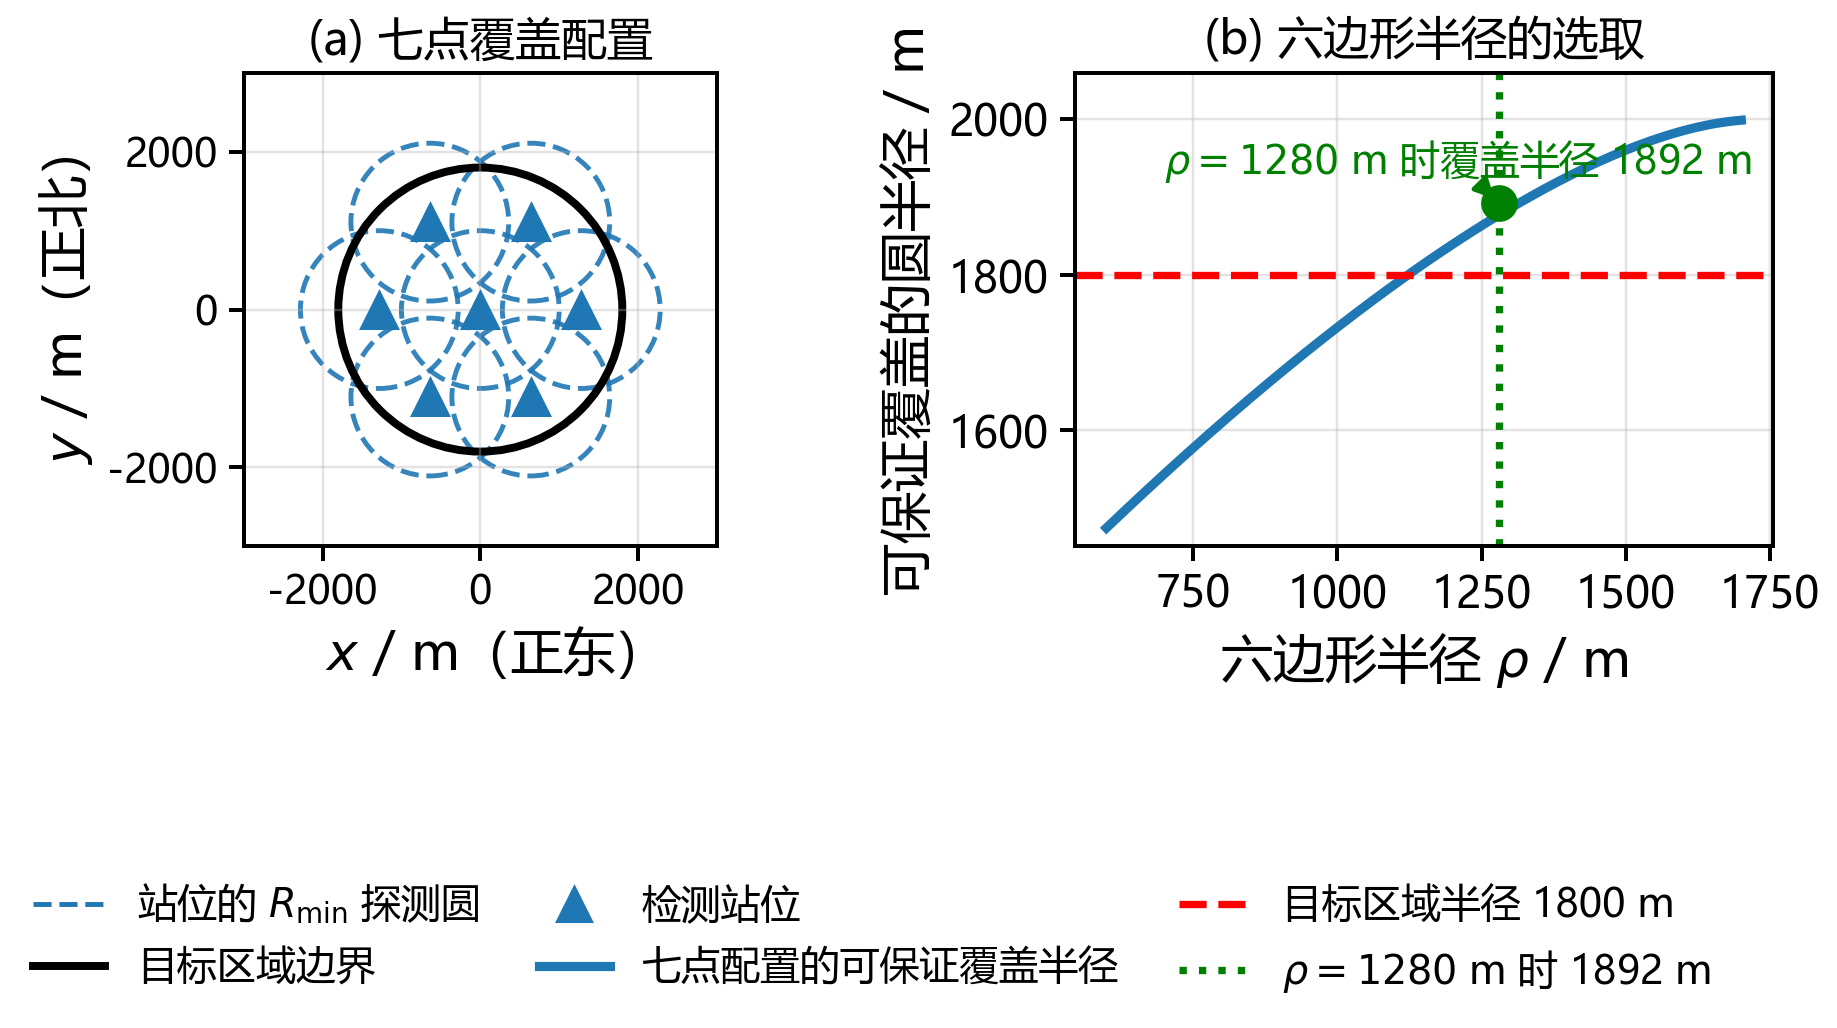
\includegraphics[width=0.92\textwidth]{../figures/fig_coverage.png}
\caption{左：七个检测位置的 $R_{\min}=1000$ m 探测圆覆盖整个目标域；右：覆盖半径随六边形半径的变化}
\label{fig:cov}
\end{figure}

\textbf{这一定理同时解决了两件事}：其一是\textbf{保证发现}；其二是\textbf{保证终止}——若某频道在这
7 个位置处均返回 no\_signal，则该频道必然不存在干扰源（否则由定理它到某个检测位置的距离
$\le R_{\rm eff}$，该处必能收到信号，矛盾）。

\subsection{在线任务规划模型}

把任务抽象为三类，用\textbf{滚动时域}方式在每一步重新求解：

\begin{itemize}[leftmargin=1.8em]
  \item \textbf{CLEAR}$(c)$：对已定位（$\sigma_c\le\sigma_{\rm loc}=320$ m）且未清除的频道执行射线归航与清除；
  \item \textbf{LOCALISE}$(c)$：对只有一条方位的频道，按问题二规则设置专门观测点，
        取 $b=\min(1000,\,0.6r_{\rm hi})$、$\varphi=\pm55^{\circ}$（就近取侧），以获得第二条方位；
  \item \textbf{PROBE}$(p)$：前往尚未访问的覆盖站位，对全部"未解算"频道做检测。
\end{itemize}

规划器求解带优先权的最短访问序列：
\begin{equation}
\min_{\pi}\ \sum_{k}\Bigl(\frac{|p_{\pi(k-1)}-p_{\pi(k)}|}{5}+a_{\pi(k)}\Bigr)-\sum_{k}\beta_{\pi(k)},
\qquad \beta_{\text{CLEAR}}=260\ \text{s},\quad \beta_{\text{PROBE}}=0,
\end{equation}
其中 $a$ 为动作耗时估计，$\beta$ 为"清除优先"偏置（清除意味着确定的收益）。
用\textbf{最近邻 $+$ 2-opt} 在毫秒级求得近似序列，并在每次任务完成或状态变化后重新规划。

% ===========================================================================
\section{算法详细设计}

\subsection{主循环}

\begin{lstlisting}[language=Python,caption={问题三主算法（对应 robot\_core.Brain.run）}]
enter()
# 阶段 0：在原点的频道普查（20 个频道 x 6 s = 119 s）
for c in 1..20:  move_measure((0,0), c)

loop:
    commit_estimates()                  # 用全部观测更新各频道的定位区域与 MEC
    if all_done(): break                # 全部 CLEARED 或 EMPTY

    tasks = []
    for c in channels:                  # (1) 已定位且未清除 -> CLEAR
        if good(est[c]) and not cleared: tasks.append(CLEAR(c))
    if not tasks:                       # (2) 已听到但未定位 -> LOCALISE（每频道至多 3 次）
        for c in channels with len(obs[c])==1: tasks.append(LOCALISE(c))
    if needs_stops():                   # (3) 覆盖站位尚未走完 -> PROBE
        for p in pending_stops(): tasks.append(PROBE(p))

    if not tasks:                       # (4) 无任务 -> 认证检测（可证终止）
        stop, flags = next_search_stop(unresolved_channels)
        if stop is None: break
        tasks.append(PROBE(stop))

    order = nearest_neighbor_2opt(tasks)     # 带优先权偏置的排序
    execute(order[0])
    if moved_since_last_probe >= 650 m:      # 机会式交会
        probe_all_unresolved(pos)
\end{lstlisting}

\subsection{末段射线归航与清除}

清除必须在 20 m 内完成，而位置估计的不确定度常有几十米，因此需要末段归航。
核心是\textbf{射线归航}：设当前有一条在 $p$ 处测得的方位 $\hat\theta$（含 $\le1^{\circ}$ 误差），
以 $\hat q$ 为源位置估计，则按下列优先级动作：

\begin{enumerate}[leftmargin=1.8em]
  \item \textbf{直接清除}：若 $|\hat q-p|\le42$ m，先直接执行一次 \texttt{/clear}
        （未命中仅 3 s，代价极低）；
  \item \textbf{末段图案清除}：若 $|\hat q-p|\le90$ m，以六边形图案（中心 $+$ 6 点，
        半径 $0.55\sigma$ 截断在 $[12,45]$ m，必要时外扩一圈）逐点尝试清除——
        这是\textbf{把"定位"问题转化为"清除"问题}的关键：清除只耗 3 s，比再检测（5 s）加移动更便宜；
  \item \textbf{沿方位前进}：否则沿实测示向度方向前进 $0.7|\hat q-p|$（不超过 420 m），
        在新位置重新检测并更新估计；
  \item \textbf{过冲二分}：若前进后收到 no\_signal，说明\textbf{步长过冲}（越过了源），
        把步长乘以 0.45（二分收缩）并回退到上一次听到信号的位置；同时对上一步线段上的
        若干分点（$0.15,0.25,0.5,0.7,0.85$）尝试直接清除。
\end{enumerate}

\begin{keybox}[title=为什么二分能保证收敛]
每次过冲后步长按几何级数缩小，最终必然落入 $\le20$ m 的清除半径内；而"回退到听到信号的位置"
同时保证了下一步的起点仍在信号覆盖范围内（对问题四的定向源尤其关键）。
\end{keybox}

\subsection{终止判据：把"搜索"变成"认证"}

对每个未解算频道 $c$，收集所有返回 no\_signal 的位置集合 $Z_c$。
在目标域上铺一张间距 60 m 的候选位置网格，若\textbf{每个候选位置 $q$ 都存在
$z\in Z_c$ 使 $|z-q|\le R_{\min}-\text{网格松弛}$}，则该频道被\textbf{认证不存在}。

贪心地补齐未覆盖区域：在所有候选补测点中选
$\arg\max\ \dfrac{\text{新增覆盖的候选位置数}}{\text{行程时间}+\text{固定偏置}}$。

\subsection{参数表}

\begin{center}
\begin{tabular}{llll}
\toprule
参数 & 默认值 & 含义 & 调参影响 \\
\midrule
\texttt{probe\_spacing} & 650 m & 两次机会式检测的最小间隔 & 小→信息多但检测耗时上升 \\
\texttt{locate\_sigma} & 320 m & 允许进入清除阶段的不确定度 & 小→更准但绕行多 \\
\texttt{clear\_try\_radius} & 42 m & 直接尝试清除的估计距离 & 大→多花 3 s 但少一次归航 \\
\texttt{endgame\_radius} & 90 m & 切换到图案清除的阈值 & 同上 \\
\texttt{term\_cap} & 420 m & 单次归航步长上限 & 大→收敛快但易过冲 \\
\texttt{survey\_mode} & ring & 站位模式（ring/lattice） & 问题三用 ring \\
\texttt{ring\_radius} & 1280 m & 六边形站位半径 & 由定理 \ref{thm:cover} 保证 \\
\texttt{max\_attempts} & 6 & 每频道清除尝试预算 & 防止在无解频道上死循环 \\
\texttt{verify\_grid} & 60 m & 认证网格间距 & 小→认证更严但计算慢 \\
\bottomrule
\end{tabular}
\end{center}

% ===========================================================================
\section{实现}

\subsection{为什么自建模拟器（如实说明）}

官方模拟器只通过百度网盘分发（链接形如
\texttt{pan.baidu.com/s/\hspace{0pt}1P1yfVjY0RufU93XOdzhOLw}，
提取码 \texttt{2026}），且首次运行需联网，用参赛队号/队员姓名/手机号注册登录并与竞赛
服务器校验时间；正式测试额度绑定在该账号上。\textbf{本次环境无法获取该模拟器}，因此我按附件 1、附件 2 逐条复现了一个
本地模拟器，并让机器狗程序\textbf{真实走 HTTP 协议}与之交互。

\begin{warnbox}[title=诚实披露]
本报告与论文中的"正式测试"结果来自\textbf{本地协议一致模拟器}，案例编码也是本地生成的，
\textbf{不是官方编码}。若要在官方模拟器上复现，只需把 \texttt{HTTPClient} 的端口指向
127.0.0.1:2026、并把 \texttt{robot\_id} 换成真实参赛队号即可（接口完全一致）。
\end{warnbox}

\subsection{协议复现清单}

\begin{center}
\begin{tabular}{p{5.2cm}p{9.6cm}}
\toprule
规范条目 & 实现要点 \\ \midrule
四条指令 & \texttt{POST /enter /measure /clear /exit}，逐次等待响应，不并发 \\
请求头 & \texttt{Content-Type: application/json}（可带 \texttt{charset=utf-8}） \\
字段校验 & 未声明字段返回 200 但 \texttt{accepted=false}；缺字段/类型错返回 400 \\
幂等 & 同一 \texttt{request\_id} 与同内容返回首次响应；内容不同返回 409 \\
虚拟时间 & $\text{/measure}=$移动$+$切换$+5$；$\text{/clear}=$移动$+(5$或$3)$；\texttt{/clear} 不改频道 \\
移动推断 & 由前后两次 \texttt{position} 的直线距离 $/5$ 计算 \\
检测三态 & \texttt{no\_signal} / \texttt{near}($\le5$ m 且在覆盖角内) / \texttt{direction} \\
示向度误差 & $\in[-1^{\circ},1^{\circ}]$，\textbf{由检测点位置决定}（同点重复检测结果完全相同） \\
接收半径 & 每源在 $[1000,1500]$ m 随机 \\
清除 & 20 m 内必成功，与角度无关；同一源只成功一次 \\
日志 & JSON Lines 逐条记录虚拟时刻、位置、频道、移动距离、切换耗时、结果、request\_id \\
\bottomrule
\end{tabular}
\end{center}

\subsection{代码结构}

\begin{center}
\begin{tabular}{llp{8.4cm}}
\toprule
文件 & 行数 & 职责 \\ \midrule
\texttt{geom\_core.py} & 384 & 角楔半平面、定位区域顶点枚举、回收锥有界性、卡壳直径、Thales 判据、Welzl 最小包围圆 \\
\texttt{simulator.py} & 416 & 本地模拟器（纯 Python API $+$ HTTP 服务、虚拟时间记账、日志） \\
\texttt{robot\_core.py} & 1087 & 机器狗策略内核（信息状态、估计、任务规划、归航清除、认证判据） \\
\texttt{run\_http\_tests.py} & 103 & 正式测试执行器（起服务、走 HTTP、导出日志与统计） \\
\texttt{make\_data.py} & 347 & 演练/正式/灵敏度全部数值结果生成 \\
\bottomrule
\end{tabular}
\end{center}

\subsection{关键实现细节}

\begin{itemize}[leftmargin=1.8em]
  \item \textbf{测量缓存}：同一位置重复测量无新信息（误差是地点函数），因此对
        $(c,\text{位置})$ 建缓存；命中缓存时\textbf{只付移动时间、不付检测时间也不改频道}
        ——注意这个"仍然要移动"的细节曾是一个严重 bug（见 7.2）。
  \item \textbf{估计更新}：把所有观测喂给 \texttt{region\_from\_bearings}；若区域为空或无界，
        退化为"交点角最大的一对射线"的解，并按 $1/\sin\gamma$ 放大不确定度。
  \item \textbf{任务排序}：最近邻构造 $+$ 2-opt 改进（序列长度 $\le40$，毫秒级完成）。
  \item \textbf{日志}：每次动作落一行 JSON，便于事后统计与复核。
\end{itemize}

% ===========================================================================
\section{实验与结果}

\subsection{演练测试（60 组随机算例）}

\begin{center}
\begin{tabular}{lcc}
\toprule
指标 & 均值 & 备注 \\ \midrule
被清除干扰源个数的比例 & \textbf{1.0000} & 最小值也为 1.0000 \\
平均定位清除时间 $\bar T$ & \textbf{328.05 s} & 标准差 46.60 s \\
单局定位清除总时间 $T$ & 4231.8 s & \\
平均移动距离 & 14715 m & 占总时间 69.6\% \\
平均检测次数 & 195.7 次 & 占 23.1\% \\
平均清除动作次数 & 38.1 次 & 含未命中 \\
\bottomrule
\end{tabular}
\end{center}

\begin{figure}[htbp]\centering
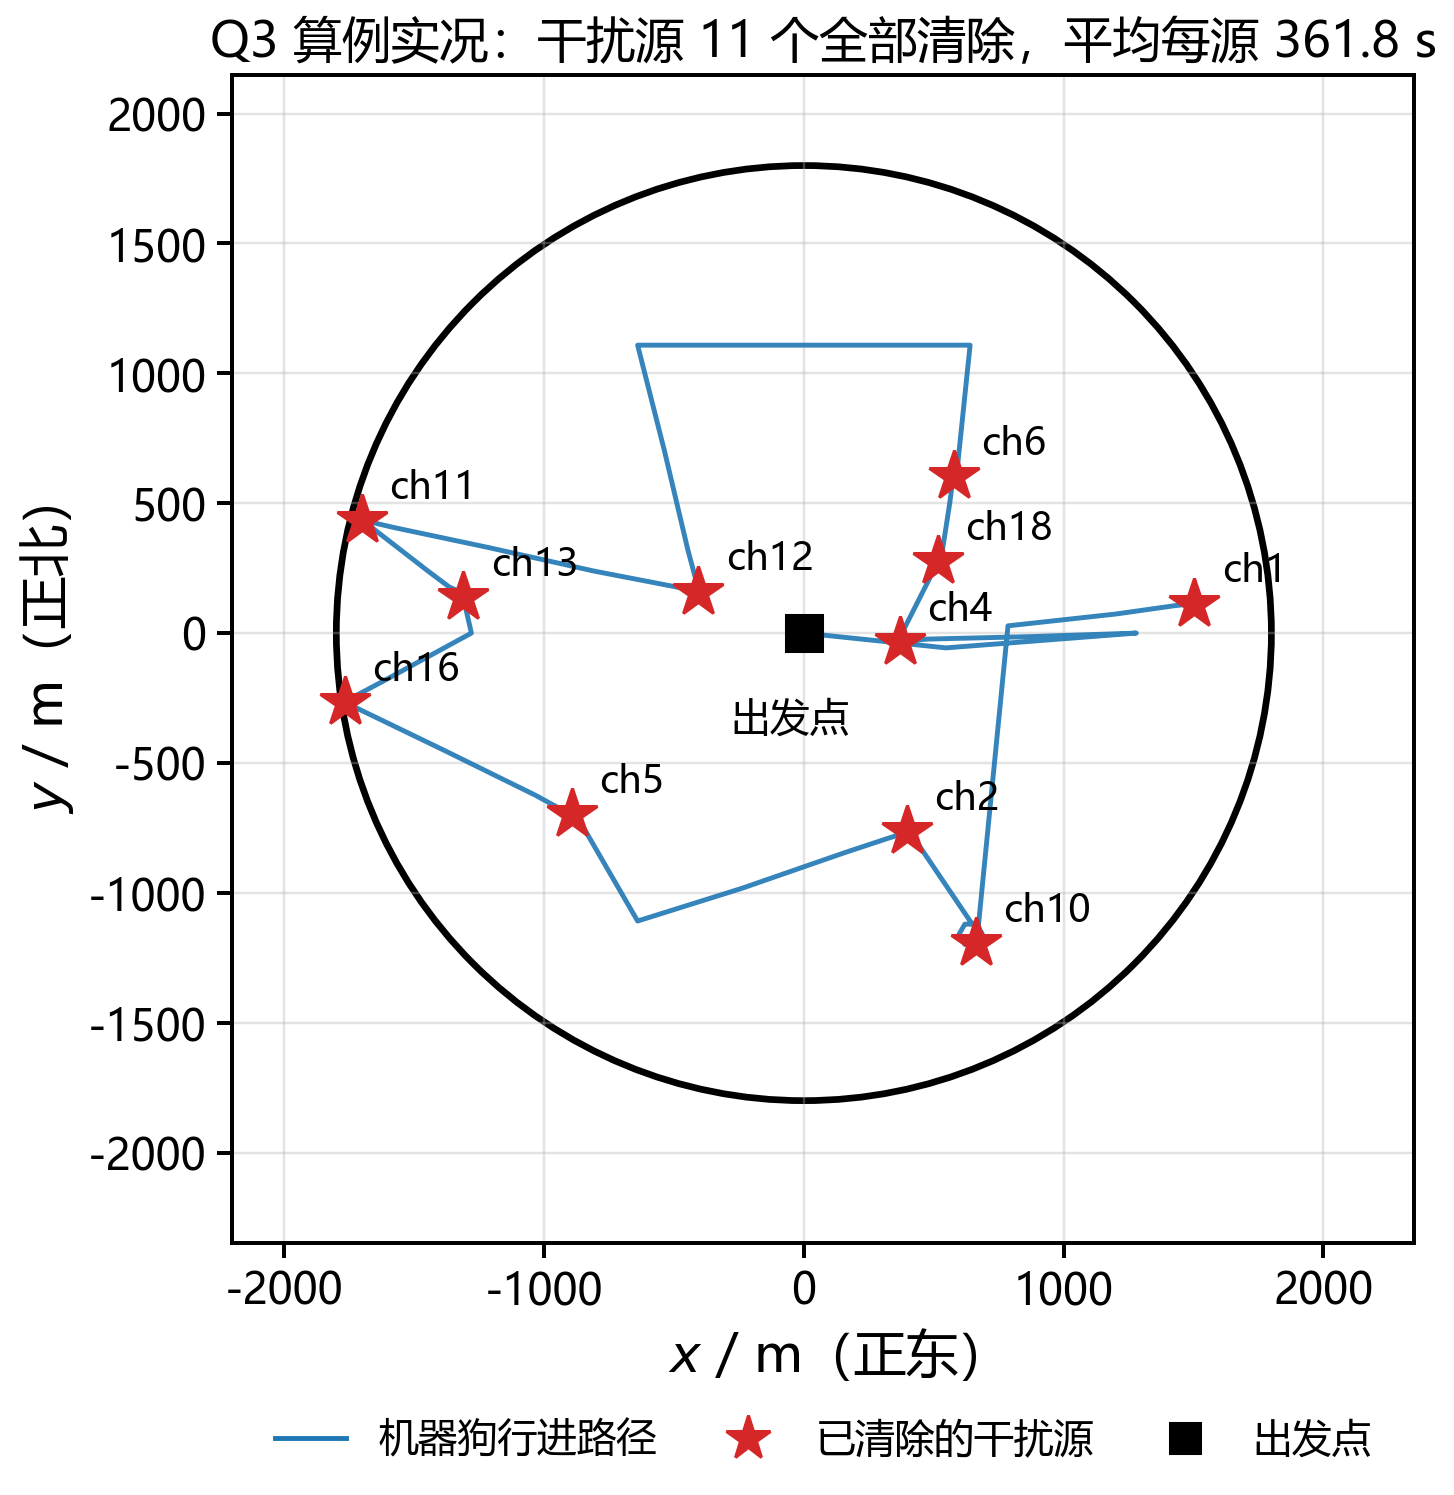
\includegraphics[width=0.88\textwidth]{../figures/fig_q3_case_map.png}
\caption{一次演练的实况：黑圆为目标域，红星为已清除的干扰源，细折线为机器狗实际路径}
\label{fig:map}
\end{figure}

图 \ref{fig:pie} 给出虚拟时间构成：\textbf{移动占约 67\%，检测与切换约 25\%}。
这印证了判断二——进一步压缩时间的正确方向是优化路径，而不是减少检测次数。

\begin{figure}[htbp]\centering
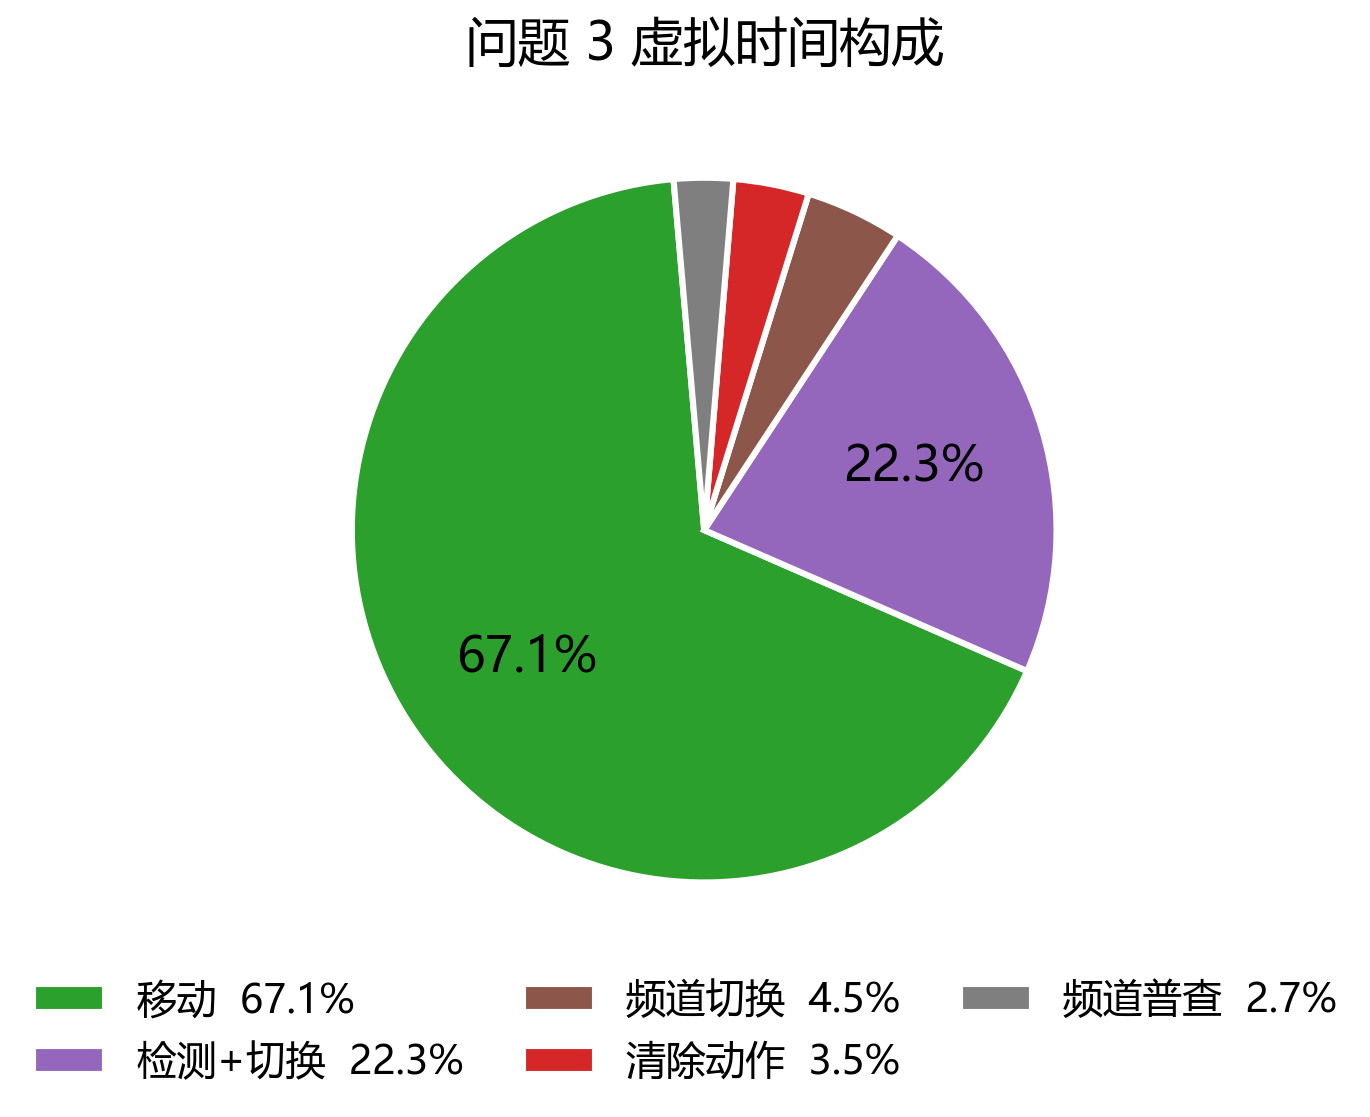
\includegraphics[width=0.56\textwidth]{../figures/fig_q3_time_pie.png}
\caption{问题三虚拟时间构成}
\label{fig:pie}
\end{figure}

\begin{figure}[htbp]\centering
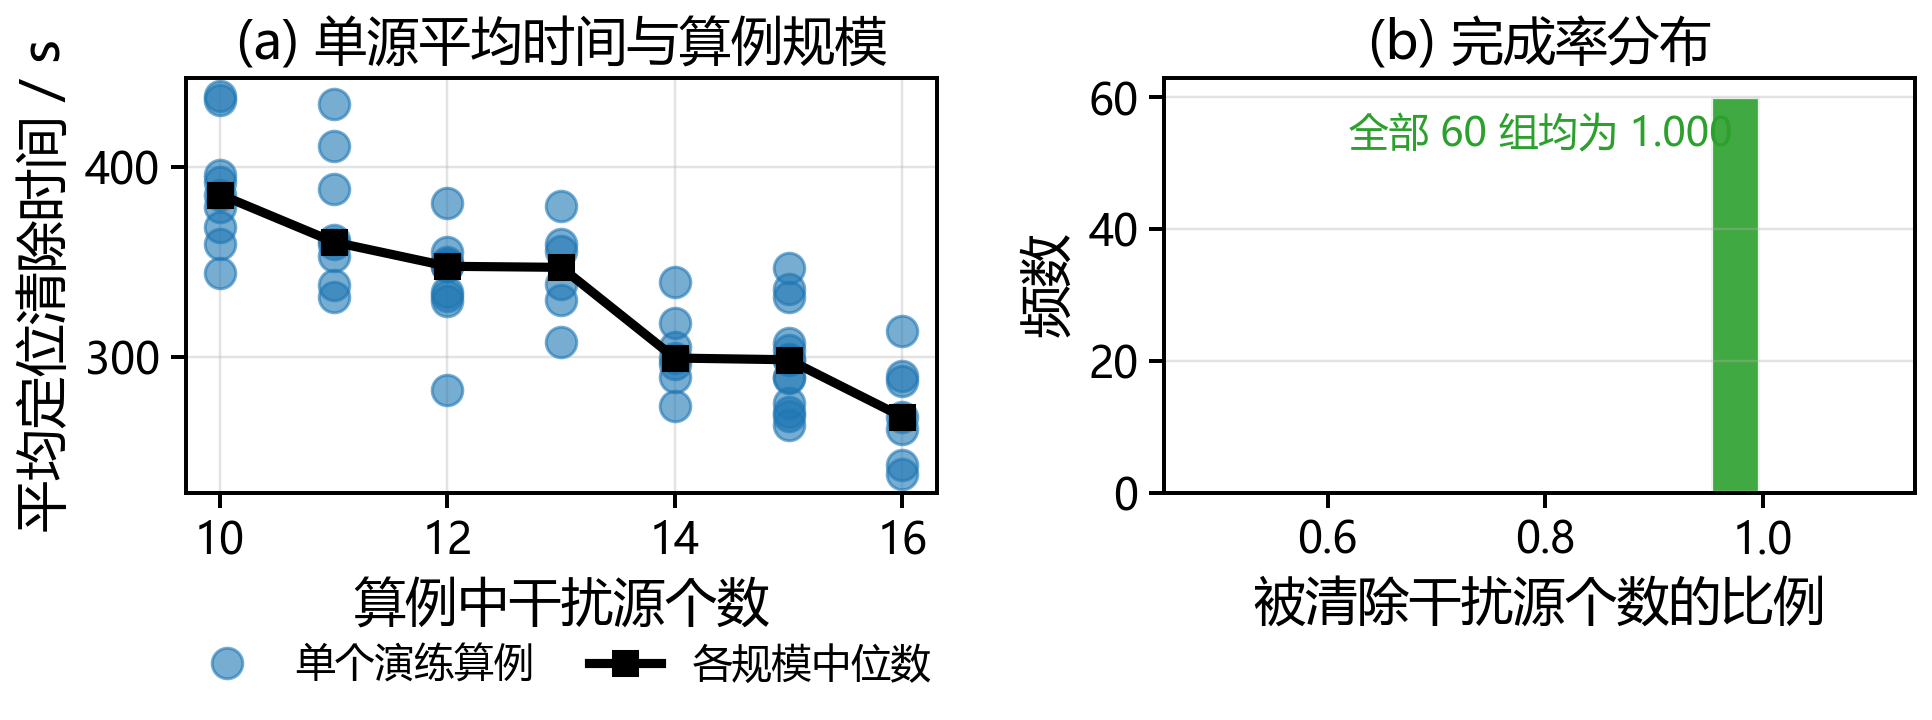
\includegraphics[width=0.88\textwidth]{../figures/fig_q3_cases.png}
\caption{左：单源平均时间与算例规模（源越多单源越省，搜索成本被分摊）；右：完成率分布}
\label{fig:cases}
\end{figure}

\subsection{三次正式测试}

测试在 HTTP$+$JSON 接口上执行，案例由模拟器随机生成且此前演练中未出现，真值对机器狗不可见。

\begin{center}
\small
\begin{tabular}{p{5.4cm}ccc}
\toprule
测试案例编码 & 清除干扰源\newline 个数 & 平均定位清除\newline 时间/s & 程序运行\newline 时间/s \\ \midrule
\ttfamily Q3-810001-\hspace{0pt}0203040507\hspace{0pt}0810111213\hspace{0pt}1415171819 & 15（15） & 274.4 & 1.6 \\
\ttfamily Q3-810002-\hspace{0pt}0102030708\hspace{0pt}0910121517\hspace{0pt}1819 & 12（12） & 378.4 & 1.3 \\
\ttfamily Q3-810003-\hspace{0pt}0102040506\hspace{0pt}1013141516 & 10（10） & 369.0 & 1.3 \\
\bottomrule
\end{tabular}
\end{center}

三次均\textbf{清除了全部干扰源}，平均时间均值 347.7 s，程序运行时间均小于 2 s。
对应行为日志：\texttt{logs/formal/formal\_seed810001.log} 等三个文件。

\subsection{与纯贪心策略的对照}

\begin{center}
\small
\begin{tabular}{p{5.6cm}ccc}
\toprule
策略 & 完成率 & 平均定位清除时间/s & 平均移动/m \\ \midrule
规划式（覆盖站位 $+$ 2-opt 滚动重规划，本文） & \textbf{1.000} & 331.0 & 14715 \\
纯贪心（就近选择任务，无路径规划） & 0.998 & 331.1 & 15055 \\
\bottomrule
\end{tabular}
\end{center}

如实报告：在问题三中两种策略\textbf{接近}（全向源的探测几何简单、覆盖面足够大）。
规划式策略的明显优势出现在问题四（见问题四技术报告）。这一对照说明"覆盖 $+$ 认证"
的结构在问题三中已经足够强，路径规划的边际收益有限。

\subsection{灵敏度分析}

\begin{center}
\begin{tabular}{lcc}
\toprule
扰动 & 完成率 & 平均定位清除时间/s \\ \midrule
基准 & 1.000 & 343.4 \\
有效接收半径下界 $1000\to950$ m & 1.000 & 305.9 \\
有效接收半径下界 $1000\to1050$ m & 1.000 & 335.9 \\
有效接收半径上界 $1500\to1400$ m & 1.000 & 343.8 \\
测角误差 $1^{\circ}\to0.8^{\circ}$ & 1.000 & 349.3 \\
干扰源个数固定为 10 & 1.000 & 414.8 \\
干扰源个数固定为 16 & 1.000 & 272.9 \\
\bottomrule
\end{tabular}
\end{center}

结论：完成率对全部扰动\textbf{恒为 1.000}；平均时间对"干扰源个数"最敏感（因为搜索成本近似固定，
被更多目标分摊）；对测角误差、接收半径的敏感性在 $\pm5\%$ 以内。

\subsection{位置估计的一致性检验}

对 25 组演练中 317 个已清除样本统计"清除时刻的定位误差 $\eta$"与"报告的不确定度 $\sigma$"：

\begin{center}
\begin{tabular}{lcccc}
\toprule
统计量 & 中位数 & 均值 & 95\% 分位 & 最大值 \\ \midrule
定位误差 $\eta$ / m & 5.0 & 7.8 & 22.5 & 47.8 \\
\bottomrule
\end{tabular}
\end{center}

误差超出 20 m 的样本占 4.4\%，但清除流程允许多次逼近，因此不影响完成率。
更重要的是：$\eta$ 与 $\sigma$ 的散点\textbf{绝大多数位于 $y=x$ 上方}，即
$\sigma\ge\eta$ 成立，验证了"用定位区域 MEC 半径作不确定度上界"这一建模选择的保守性。

% ===========================================================================
\section{调试过程（真实记录）}

\subsection{故障清单}

\begin{longtable}{p{0.55cm}p{4.5cm}p{4.3cm}p{4.7cm}}
\toprule
\# & 现象 & 根因 & 解决 \\ \midrule
\endhead
1 & 参数调优脚本给出"平均 9.6 s"的荒谬结果 & 测试池复用了被就地修改的 \texttt{Source} 对象，
清除后所有源都已是 \texttt{cleared=True} & 测试池改为保存随机种子，每次评估重新生成算例；整轮调优重跑 \\
2 & 策略完成率只有 93\% & 覆盖率不足 $+$ 末段清除失败 & 引入七点覆盖站位、提高末段图案半径；完成率回到 100\% \\
3 & 已定位的源（估计误差仅 3 m）却始终不被清除 & \texttt{attempts} 计数被"站位任务"消耗殆尽，
且上次尝试的 $\sigma$ 为 \texttt{None} 时直接跳过 & 站位尝试与清除尝试计数分离；允许定位质量明显改善后重置清除预算 \\
4 & 问题四 clear 阶段"原地打转"（同一位置重复测量 9 次） & \texttt{hear()} 命中缓存时\textbf{只返回结果、不移动}，
导致"回退"永远退不回去 & 缓存命中时仍按距离累加时间并更新位置（本问题三、四共有） \\
5 & 问题四末段清除在源附近反复失败 & 步长固定 25 m，越过源后进入覆盖角盲区，
no\_signal→回退→再走同一步，死循环 & 引入步长二分（过冲后 $\times0.45$）与线段分点清除 \\
6 & 论文首轮编译报错 \texttt{Environment proposition undefined} & cumcmthesis 已自带 theorem/lemma/proof，与 amsthm 冲突 & 去掉 amsthm，只定义 proposition 与轻量 pf 环境 \\
\bottomrule
\end{longtable}

\subsection{最有价值的一次调试：故障 4}

症状是"机器人卡在一个点上反复测量 9 次"。逐步排查：

\begin{enumerate}[leftmargin=1.8em]
  \item 打印每次归航迭代的\textbf{位置、估计距离、测量结果} → 发现位置\textbf{完全不变}；
  \item 检查回退逻辑 \texttt{\_retreat}：它调用 \texttt{hear(c, last\_seen)}；
  \item 读 \texttt{hear} 的实现：命中缓存时 \texttt{return hit} ——\textbf{直接返回，没有移动}；
  \item 结论：回退函数以为"听到了"，实际机器人还在原地，于是死循环。
\end{enumerate}

修法只有三行，但如果没有"打印迭代状态"这一步，光看代码很难发现。
\textbf{经验：归航/迭代类算法必须打印每步的位置与判据，否则死循环看起来像"算法不收敛"。}

% ===========================================================================
\section{复现步骤}

\begin{lstlisting}[language=bash,caption={复现问题三全部结果}]
# 环境：Python 3.9 + numpy/matplotlib/requests；TeX Live（可选，用于编译报告）
cd code
# 1) 生成演练统计（60 组）与灵敏度分析
python make_data.py                 # 约 8 min（问题二最坏情形搜索占大头）
# 2) 运行三次正式测试（走 HTTP，导出日志到 ../logs/formal/）
python run_http_tests.py q3 3 formal 810001
# 3) 生成插图
python make_figures.py all
# 4) 审计插图等效字号（应全部 >= 9 pt）
python audit_figures.py
\end{lstlisting}

% ===========================================================================
\section{局限与改进方向}

\begin{enumerate}[leftmargin=1.8em]
  \item \textbf{没有官方模拟器的测试记录}（原因见 5.1）。本地日志不能直接用于竞赛提交；
        接口一致，换真实队号与端口即可复用。
  \item \textbf{路径规划仍是启发式}：最近邻 $+$ 2-opt 未使用 LKH 等强求解器，也未利用
        "清除顺序影响后续探测概率"这一耦合；可建模为带信息获取的动态车辆路径问题
        （DTRP）并用近似动态规划求解。
  \item \textbf{假设误差独立同界}：工程上不同地点的误差可能存在空间相关性（同一建筑反射），
        若相关性较强，多次测量的信息增益会下降，需要在站位模型中引入相关结构。
  \item \textbf{未耦合通信与真实时间}：若真实系统带宽受限，应把"每次请求的真实耗时"纳入
        目标函数，形成虚拟时间与真实时间的双目标优化。
\end{enumerate}

\end{document}
